% Fig. 1 -- Epistemic trust as inference about other minds (Section 2). Pure TikZ; build: xelatex.
% Each component of epistemic trust is one labelled structure; numbered badges mark where the four
% routes to disrupted trust act (Section 3). No hue: colour is reserved for entities in this paper.
\documentclass[border=0pt]{standalone}
% figstyle.tex -- shared style for all figures of "Epistemic Trust as Inference About Other Minds".
% Compile each figure with xelatex (standalone class). Full-width figures are exactly 504pt wide,
% the \textwidth of the Frontiers template, so they are included at 100% and never rescaled.
%
% Colour roles (validated with the dataviz skill's validate_palette.js on a white surface):
%   groups   : controls = slot 1 blue #2a78d6, BPD = slot 2 orange #eb6834 (all-pairs PASS)
%   stances  : trusting = green #008300, mistrusting = violet #6250d6 (all-pairs PASS; tritan 7.6,
%              so always paired with a second cue: dash for rigid stances, plus labels)
%   models   : theoretical curves in primary ink (no hue, so hues stay reserved for entities)
%   chrome   : ink #0b0b0b / #52514e / #898781, gridline #e1e0d9, axis #c3c2b7 (reference palette)

\usepackage{fontspec}
% Fonts are loaded by file name: XeTeX then finds them in TeX Live without system registration.
\setmainfont{texgyreheros}[Extension=.otf, UprightFont=*-regular, BoldFont=*-bold,
  ItalicFont=*-italic, BoldItalicFont=*-bolditalic]
\setsansfont{texgyreheros}[Extension=.otf, UprightFont=*-regular, BoldFont=*-bold,
  ItalicFont=*-italic, BoldItalicFont=*-bolditalic]
\renewcommand{\familydefault}{\sfdefault}
\hyphenpenalty=10000 \exhyphenpenalty=10000   % figures never hyphenate
\usepackage{unicode-math}
\setmathfont{FiraMath-Regular.otf}[Scale=MatchLowercase]   % sans-serif math to match the text

\usepackage{tikz}
\usetikzlibrary{positioning,calc,fit,backgrounds,arrows.meta}
\usepackage{pgfplots}
\pgfplotsset{compat=1.18}
\usepgfplotslibrary{groupplots,fillbetween}

% ---- colours ---------------------------------------------------------------
\definecolor{inkPrimary}{HTML}{0B0B0B}
\definecolor{inkSecondary}{HTML}{52514E}
\definecolor{inkMuted}{HTML}{898781}
\definecolor{gridLine}{HTML}{E1E0D9}
\definecolor{axisLine}{HTML}{C3C2B7}
\definecolor{bandFill}{HTML}{F0EFEC}
\definecolor{groupControls}{HTML}{2A78D6}
\definecolor{groupBPD}{HTML}{EB6834}
\definecolor{stanceTrust}{HTML}{008300}
\definecolor{stanceMistrust}{HTML}{6250D6}

% ---- type sizes (true size: figures are never rescaled) --------------------
\newcommand{\figfont}{\fontsize{8}{9.6}\selectfont}
\newcommand{\ticksize}{\fontsize{7}{8.4}\selectfont}
\newcommand{\panelfont}{\fontsize{9}{10.8}\selectfont\bfseries}

% ---- line weights -----------------------------------------------------------
\tikzset{
  hairline/.style={line width=0.4pt},
  dataline/.style={line width=1.3pt, line cap=round, line join=round},
  rigid/.style={dash pattern=on 3.2pt off 2.2pt},
  panel label/.style={font=\panelfont, text=inkPrimary, anchor=north west, inner sep=0pt},
  note/.style={font=\ticksize, text=inkSecondary, inner sep=1pt},
}

% ---- row filter: plot only the rows whose column #1 equals #2 (e.g. group = BPD) ----
\pgfplotsset{
  only rows/.style 2 args={
    unbounded coords=discard,
    x filter/.append code={%
      \edef\figRowValue{\thisrow{#1}}\edef\figWanted{#2}%
      \ifx\figRowValue\figWanted\else\def\pgfmathresult{inf}\fi},
  },
  group dots/.style={only marks, mark=*, mark size=1.75pt,
    mark options={draw=white, line width=0.5pt, fill=#1}, color=#1},
}

% ---- the shared axis style --------------------------------------------------
\pgfplotsset{
  paper axis/.style={
    scale only axis,
    axis lines*=left,
    axis line style={axisLine, line width=0.4pt},
    every tick/.style={axisLine, line width=0.4pt},
    tick align=outside,
    major tick length=2.5pt,
    minor tick length=1.5pt,
    tick label style={font=\ticksize, text=inkSecondary},
    label style={font=\figfont, text=inkPrimary},
    title style={font=\figfont, text=inkPrimary, align=center},
    grid=major,
    major grid style={gridLine, line width=0.4pt},
    clip mode=individual,
    legend style={draw=none, fill=none, font=\ticksize, text=inkSecondary},
    legend cell align=left,
    every axis plot/.append style={dataline},
  },
}

\newcommand{\sub}{\ticksize\color{inkSecondary}}
\tikzset{
  box/.style={draw=axisLine, line width=0.5pt, fill=white, rounded corners=3pt, align=center,
              font=\figfont, text=inkPrimary, inner sep=4pt, minimum height=26pt},
  sub/.style={font=\ticksize, text=inkSecondary},
  flow/.style={-{Stealth[length=4.5pt, width=4pt]}, line width=0.7pt, draw=inkSecondary},
  infer/.style={-{Stealth[length=4.5pt, width=4pt]}, line width=0.9pt, draw=inkPrimary, dash pattern=on 3pt off 2pt},
  hier/.style={-{Stealth[length=4pt, width=3.6pt]}, line width=0.6pt, draw=inkMuted},
  comp/.style={font=\figfont\bfseries, text=inkPrimary, inner sep=1pt},
  compsub/.style={font=\ticksize, text=inkSecondary, inner sep=1pt, align=center},
  edgelab/.style={font=\ticksize, text=inkSecondary, fill=white, inner sep=1pt},
  route/.style={circle, fill=inkPrimary, text=white, font=\fontsize{6.5}{7}\selectfont\bfseries,
                inner sep=0pt, minimum size=10pt},
}

\begin{document}
\figfont
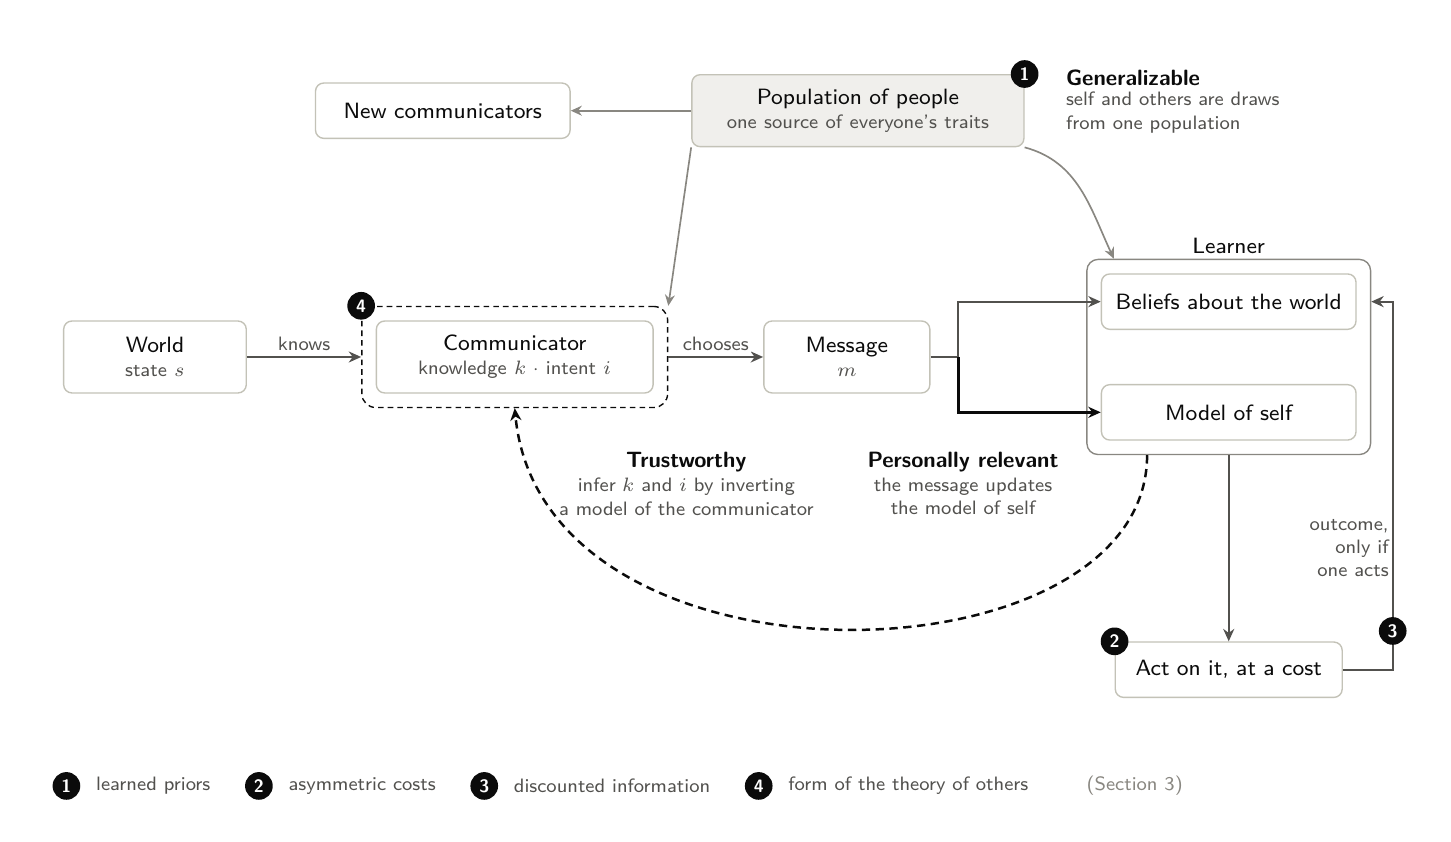
\begin{tikzpicture}
  \useasboundingbox (0,0) rectangle (504pt,284pt);

  % ---------------- generalizable: one population (top band) ----------------
  \node[box, text width=112pt, fill=bandFill] (P) at (300pt,254pt) {Population of people\\[-1pt]{\sub one source of everyone's traits}};
  \node[box, text width=84pt, minimum height=20pt] (N) at (150pt,254pt) {New communicators};
  \node[comp, anchor=north west] (G) at (374pt,270pt) {Generalizable};
  \node[compsub, anchor=north west, align=left] at (G.south west) {self and others are draws\\from one population};

  % ---------------- generative chain (middle band) ----------------
  \node[box, text width=58pt] (W) at (46pt,165pt) {World\\[-1pt]{\sub state \(s\)}};
  \node[box, text width=92pt] (C) at (176pt,165pt) {Communicator\\[-1pt]{\sub knowledge \(k\) \(\cdot\) intent \(i\)}};
  % form of the theory: what a communicator can be (dashed frame, route 4)
  \node[draw=inkPrimary, dash pattern=on 2pt off 1.5pt, line width=0.5pt, rounded corners=5pt,
        inner sep=5pt, fit=(C)] (Cform) {};
  \node[box, text width=52pt] (M) at (296pt,165pt) {Message\\[-1pt]{\sub \(m\)}};
  \node[box, text width=84pt, minimum height=20pt] (L1) at (434pt,185pt) {Beliefs about the world};
  \node[box, text width=84pt, minimum height=20pt] (L2) at (434pt,145pt) {Model of self};
  \node[draw=inkMuted, line width=0.5pt, rounded corners=4pt, inner sep=5pt, fit=(L1)(L2)] (L) {};
  \node[font=\figfont, text=inkPrimary, anchor=south, inner sep=1.5pt] at (L.north) {Learner};

  \draw[flow] (M.east) -- ++(10pt,0) |- (L1.west);
  \draw[flow, line width=1.2pt, draw=inkPrimary] (M.east) ++(10pt,0) |- (L2.west);

  \draw[hier] (P.south west) -- (Cform.north east);
  \draw[hier] (P.south east) to[out=-15, in=115] ([xshift=10pt]L.north west);
  \draw[hier] (P.west) -- (N.east);


  \draw[flow] (W) -- node[edgelab, above=1pt] {knows} (Cform.west |- W);
  \draw[flow] (Cform.east |- M) -- node[edgelab, above=1pt] {chooses} (M);

  % ---------------- trustworthy: inverting the communicator (lower band) ----------------
  \draw[infer] ([xshift=22pt]L.south west) .. controls ([xshift=22pt]L.south west |- 0,46pt) and (186pt,40pt) .. (Cform.south);
  \node[comp, anchor=north] (T) at (238pt,132pt) {Trustworthy};
  \node[compsub, anchor=north] at (T.south) {infer \(k\) and \(i\) by inverting\\a model of the communicator};

  % ---------------- personally relevant: the message reaches the self ----------------
  \node[comp, anchor=north] (R) at (338pt,132pt) {Personally relevant};
  \node[compsub, anchor=north] at (R.south) {the message updates\\the model of self};

  % ---------------- the acting loop ----------------
  \node[box, text width=74pt, minimum height=20pt] (A) at (434pt,52pt) {Act on it, at a cost};
  \draw[flow] (L.south) -- (A.north);
  \draw[flow] (A.east) -- ++(18pt,0) |- ([yshift=0pt]L.east |- L1);
  \node[compsub, anchor=east, align=right] at (493pt,96pt) {outcome,\\only if\\one acts};

  % ---------------- route badges ----------------
  \node[route] at (P.north east) {1};
  \node[route] at (A.north west) {2};
  \node[route] at ([xshift=18pt, yshift=14pt]A.east) {3};
  \node[route] at (Cform.north west) {4};

  % ---------------- key to the routes ----------------
  \node[route] (k1) at (14pt,10pt) {1};  \node[sub, anchor=west] (t1) at ([xshift=2pt]k1.east) {learned priors};
  \node[route] (k2) at ([xshift=14pt]t1.east) {2}; \node[sub, anchor=west] (t2) at ([xshift=2pt]k2.east) {asymmetric costs};
  \node[route] (k3) at ([xshift=14pt]t2.east) {3}; \node[sub, anchor=west] (t3) at ([xshift=2pt]k3.east) {discounted information};
  \node[route] (k4) at ([xshift=14pt]t3.east) {4}; \node[sub, anchor=west] (t4) at ([xshift=2pt]k4.east) {form of the theory of others};
  \node[sub, anchor=west, text=inkMuted] at ([xshift=14pt]t4.east) {(Section~3)};
\end{tikzpicture}
\end{document}
